\section{Experiment}
\label{sec:experiment}
%
The simulation experiments we run in Gymnasium supports the theoretical
computation performed in Section~\ref{ssec:prob_sol}. The Monte Carlo
simulations that we perform can yield even more results, such as what is the 
expected number of ``bad'' moves that the robot makes before it reaches the goal. Here, a bad move means that the agent moves away from the goal. We can 
further compute a histogram of the states visited, and the rewards collected on 
average.

The first result in Figure~\ref{fig:running_avg} shows the running average
number of steps taken to reach the goal over $50,000$ independent Monte Carlo
simulation runs.
%
\begin{figure}[t]
    \centering
    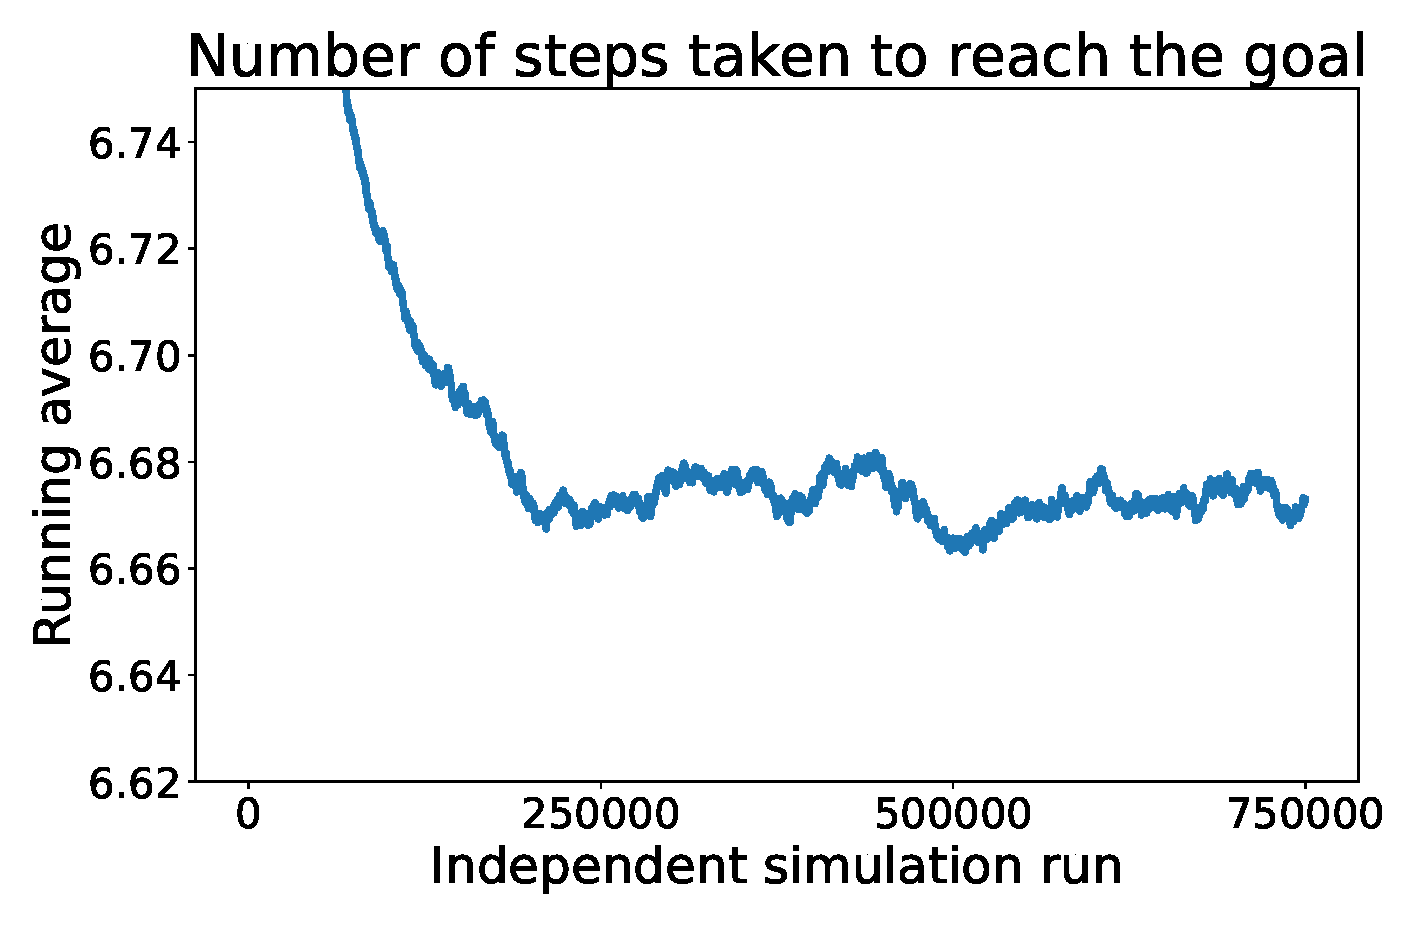
\includegraphics[width=0.5\textwidth]{./figures/running_avg.eps}
    \caption{Running average number of steps taken to reach the goal over $50,000$ independent Monte Carlo simulation runs.}
    \label{fig:running_avg}
\end{figure}
%
Figure~\ref{fig:running_avg} shows that the running average converges to $6.\bar{6}$ just as the theoretical computation indicated in Section~\ref{ssec:prob_sol}.

Figure~\ref{fig:histogram} shows the histogram of number of steps it took to 
solve the environment over $50,000$ independent Monte Carlo simulation runs. We 
observe that it takes $4$ steps to solve the environment $16.\bar{6}\%$ of the time, $6$ steps $33.\bar{3}\%$ of the time, and $8$ steps $50\%$ of the time, yielding an expected value of 
%
\[
\frac{1}{6} \times 4 + \frac{1}{3} \times 6 + \frac{1}{2} \times 8 = \frac{20}{3} = 6.\bar{6}.
\]
%
\begin{figure}[tbh]
    \centering
    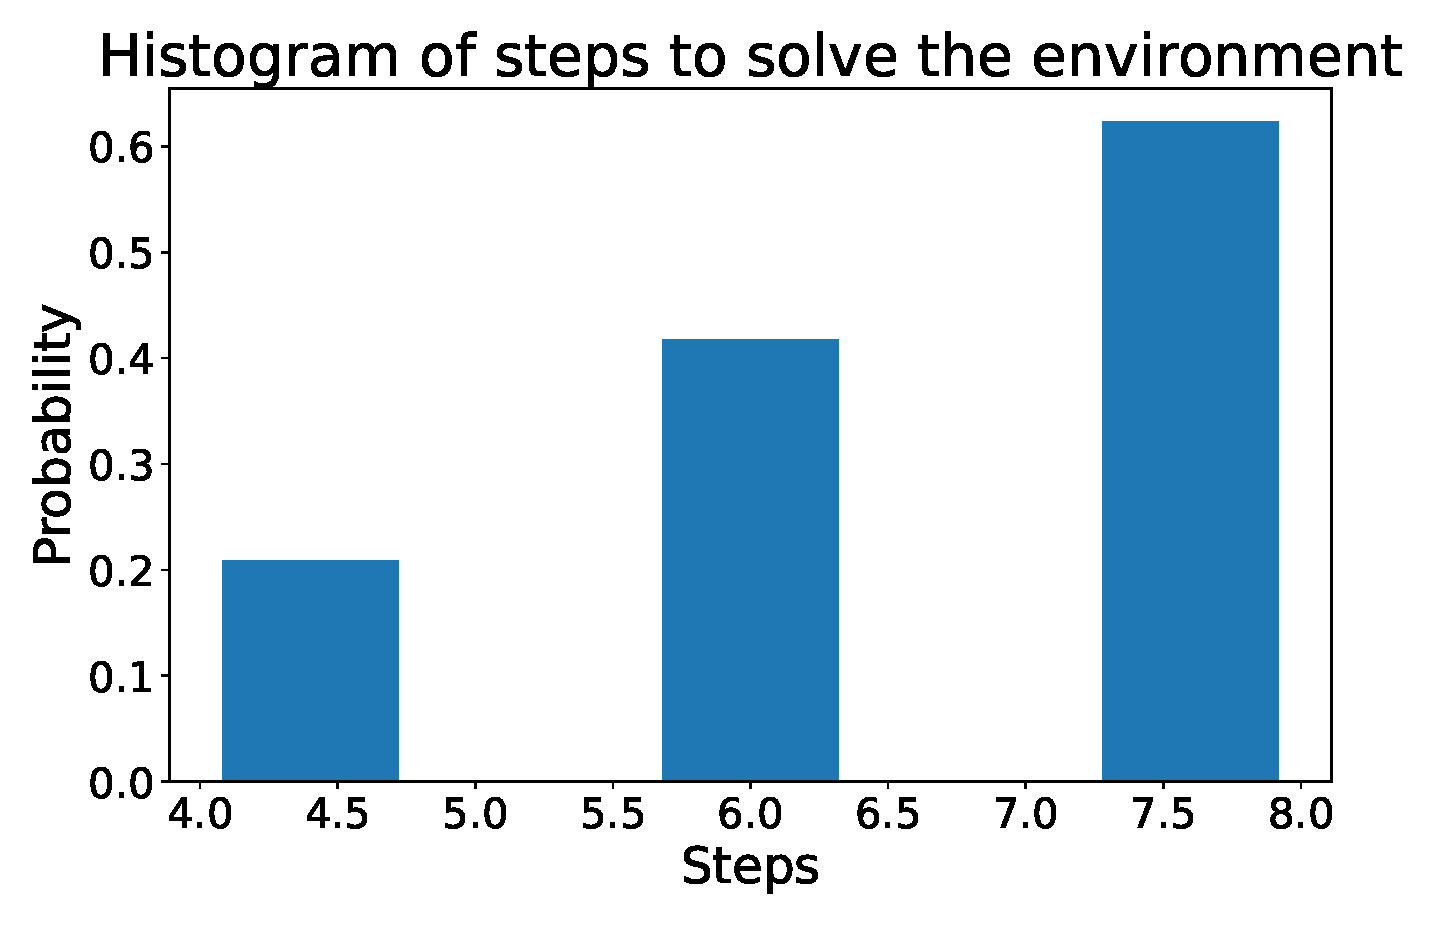
\includegraphics[width=0.5\textwidth]{./figures/steps_histogram.eps}
    \caption{Histogram of number of steps taken to solve the environment over $50,000$ independent Monte Carlo simulation runs.}
    \label{fig:histogram}
\end{figure}

Figure~\ref{fig:visit_count} shows the frequency of visits of each state under
the optimal policy deduced by $Q$-learning over $50,000$ independent Monte Carlo
runs. Notice that the ratio of the goal state being visited to the number of
runs is $1$, meaning that all runs end at the goal state.
%
\begin{figure}[bth]
    \centering
    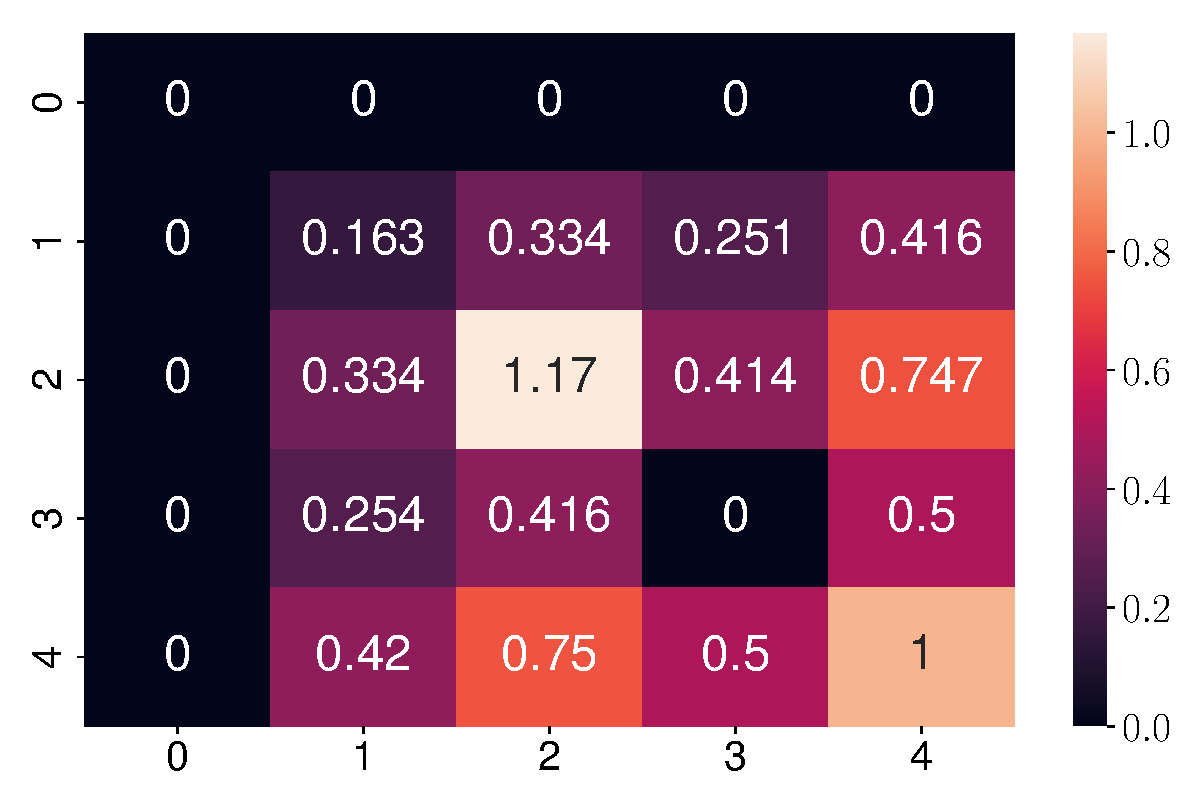
\includegraphics[width=0.5\textwidth]{./figures/visit_count_ratio.eps}
    \caption{Ratio of times a given state is visited under the optimal policy over $50,000$ independent Monte Carlo simulation runs.}
    \label{fig:visit_count}
\end{figure}

Figure~\ref{fig:bandit_scores} shows the scores each world belief achieves over
simulation steps during a single run. At the end there are four bandit
arms(world beliefs) that have the same high score of $1$, however, two of these
bandits arms have been identified to swap the ``down'' and ``right'' actions.
Since this swapping does not affect the performance of the agent, their score
matches the other two top bandit arms which have not been differentiated.
%
\begin{figure}[bth]
    \centering
    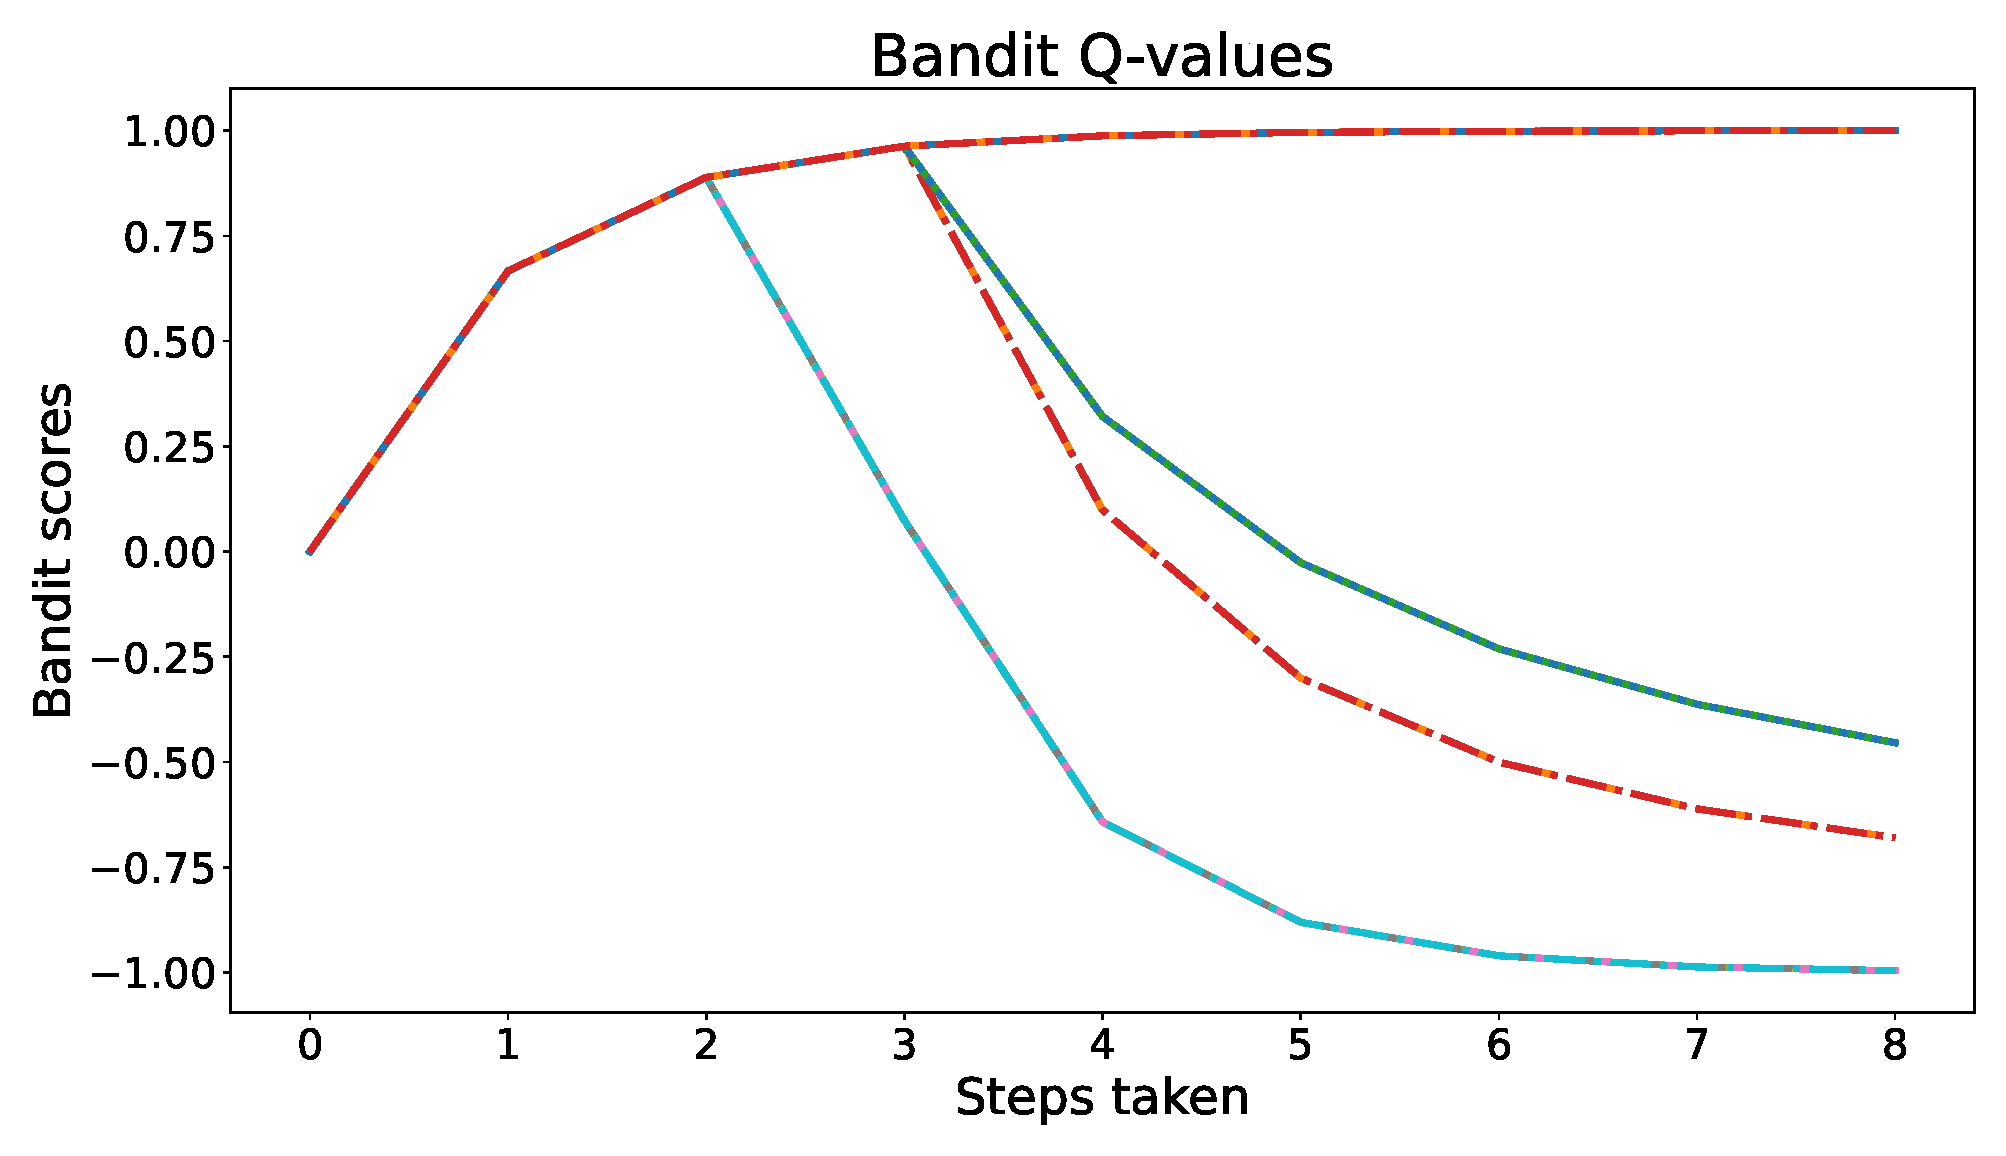
\includegraphics[width=0.5\textwidth]{./figures/bandit_scores.eps}
    \caption{Scores each world belief achieves over a single run sample.}
    \label{fig:bandit_scores}
\end{figure}